\section{Token Otorisasi}
\label{sec:token-otorisasi}

\subsection{JSON Web Token}
\label{subsec:json-web-token}

JSON Web Token (JWT) adalah format token yang ringkas dan \textit{URL-safe} untuk merepresentasikan klaim yang dipertukarkan antara dua pihak \autocite{jones2015jwt}. Klaim pada JWT direpresentasikan dalam bentuk objek JSON dan dapat diamankan menggunakan JSON Web Signature (JWS) atau JSON Web Encryption (JWE). Dengan demikian, JWT dapat digunakan untuk membawa informasi seperti identitas pengguna, peran, cakupan akses, waktu penerbitan, dan waktu kedaluwarsa token.

Secara umum, JWT terdiri dari tiga bagian utama, yaitu \textit{header}, \textit{payload}, dan \textit{signature}. Ketiga bagian tersebut dikodekan menggunakan \texttt{Base64URL} dan dipisahkan dengan tanda titik. Bentuk umum JWT dapat dituliskan sebagai berikut:

\begin{equation*}
	JWT = header.payload.signature
\end{equation*}

Bagian \textit{header} berisi informasi mengenai tipe token dan algoritma kriptografi yang digunakan. Bagian \textit{payload} berisi klaim yang menyatakan informasi mengenai subjek atau hak akses. Bagian \textit{signature} digunakan untuk memastikan integritas token sehingga perubahan pada \textit{header} atau \textit{payload} dapat terdeteksi oleh pihak yang memverifikasi token.

\subsection{PASETO}
\label{subsec:paseto}

PASETO atau \textit{Platform-Agnostic Security Tokens} adalah format token yang dirancang sebagai alternatif terhadap JWT dengan pendekatan kriptografi yang lebih terarah \autocite{arciszewski2022paseto}. Seperti JWT, PASETO digunakan untuk merepresentasikan klaim dalam bentuk token yang ringkas dan dapat dipertukarkan antar pihak. Namun, PASETO membatasi pilihan algoritma kriptografi berdasarkan versi dan tujuan penggunaan token, sehingga mengurangi risiko kesalahan konfigurasi algoritma yang dapat terjadi pada token berbasis JWT.

Secara umum, token PASETO $P$ dapat direpresentasikan sebagai:

\begin{equation*}
	P = version.purpose.message[.footer]
\end{equation*}

$version$ menunjukkan versi PASETO, $purpose$ menunjukkan tujuan penggunaan token , $message$ adalah \textit{payload} yang telah diproses secara kriptografis, dan $footer$ adalah \textit{footer} opsional. Nilai $purpose$ dapat berupa \texttt{local} atau \texttt{public}. Nilai \texttt{local} digunakan ketika isi token perlu dienkripsi menggunakan kunci simetris, sedangkan nilai \texttt{public} digunakan ketika token perlu ditandatangani menggunakan kriptografi kunci publik.

Keunggulan PASETO terletak pada desainnya yang lebih \textit{opinionated} dibandingkan JWT, terutama dalam pemilihan algoritma kriptografi. Dengan membatasi pilihan algoritma, PASETO berupaya mengurangi fleksibilitas yang berpotensi menimbulkan kesalahan implementasi. Namun, dari sisi model otorisasi, PASETO tetap berperan sebagai token pembawa klaim. Artinya, pembatasan akses seperti peran, cakupan, dan waktu berlaku tetap perlu didefinisikan pada saat token diterbitkan.

\subsection{Macaroons}
\label{sec:macaroons}

Macaroon adalah \textit{credential} otorisasi berbasis \textit{bearer} yang mendukung delegasi terdesentralisasi dalam sistem terdistribusi \autocite{birgisson2014macaroons}. Keunggulan utama Macaroon terletak pada penggunaan \textit{chained-HMAC}, yang memungkinkan proses delegasi bersifat terdesentralisasi secara efisien serta mendukung penambahan syarat \textit{caveat} yang sesuai dengan konteks penggunaan.

\subsubsection{Struktur Macaroon}
\label{subsec:struktur-macaroon}

Sebuah Macaroon $M$ didefinisikan dengan struktur:

\begin{equation*}
	M = (id, \, \mathrm{location}, \, \vec{c}, \, \mathrm{sig})
\end{equation*}

$id$ adalah pengidentifikasi unik, $location$ adalah alamat layanan target, $\vec{c} = (c_1, c_2, \dots, c_n)$ adalah daftar \textit{caveat}, dan $sig$ adalah tanda tangan \autocite{birgisson2014macaroons}. Tanda tangan ($sig$) dihitung secara rekursif untuk menjamin integritas setiap penambahan batasan (\textit{caveat}):

\begin{align*}
	sig_0 & = \text{HMAC}(RootKey, id)    \\
	sig_n & = \text{HMAC}(sig_{n-1}, c_n)
\end{align*}

$RootKey$ adalah kunci rahasia yang digunakan untuk membangkitkan token Macaroon awal. Struktur ini memungkinkan pemegang Macaroon (misalnya: Dokter A) menambahkan \textit{caveat} baru $c_{new}$ (misalnya: \texttt{time < 24h}) dan menghasilkan $sig_{new}$ untuk diberikan ke pihak lain (misalnya: Dokter B), tanpa mengetahui $RootKey$ yang asli. Kemampuan untuk menambahkan batasan baru pada token secara lokal tanpa melibatkan penerbit awal ini disebut dengan \textit{offline attenuation}. Mekanisme ini memungkinkan delegasi terdesentralisasi yang aman dan fleksibel. Gambaran mengenai delegasi dan atenuasi kewenangan melalui \textit{caveats} dapat dilihat pada Gambar \ref{fig:delegasi-macaroon}.

\begin{figure}[ht]
	\centering
	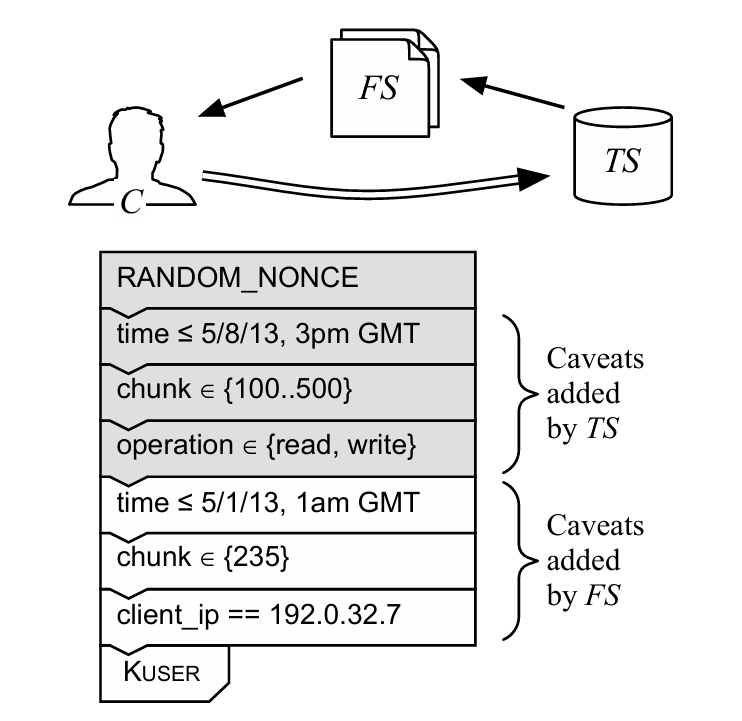
\includegraphics
	[width=0.8\textwidth]{resources/chapter-2/macaroons.png}
	\caption{Contoh delegasi dan atenuasi kewenangan pada Macaroon. C memegang Macaroon yang diturunkan dari \textit{service} FS untuk mengakses data pada \textit{service} TS dengan batasan waktu, lokasi IP, dan target data yang spesifik. \autocite{birgisson2014macaroons}}
	\label{fig:delegasi-macaroon}
\end{figure}

\subsubsection{Arsitektur Macaroons}
\label{subsec:arsitektur-macaroons}

Arsitektur Macaroons terdiri dari tiga komponen kunci: \textit{first-party caveats} yang diverifikasi oleh layanan target, \textit{third-party caveats} yang diverifikasi oleh layanan \textit{discharge} eksternal, dan struktur \textit{HMAC} berantai yang mengikat semua \textit{caveat} bersama-sama \autocite{birgisson2014macaroons}. Desain ini memungkinkan pembatasan otoritas yang fleksibel, menentukan bagaimana, oleh siapa, dan dalam konteks apa hak akses dapat dieksekusi.

\textit{First-party caveat} adalah syarat/ketentuan yang bisa diverifikasi langsung oleh pihak yang memegang kunci rahasia Macaroon (biasanya \textit{resource server} atau \textit{authorization server} yang menerbitkan token) \autocite{birgisson2014macaroons}. Bentuknya biasanya sebuah predikat/kondisi seperti \texttt{user = 123}, \texttt{expires < t}, atau \texttt{method = GET} yang dapat dicek secara lokal ketika \textit{request} datang.

\textit{Third-party caveat} adalah syarat yang tidak bisa diverifikasi langsung oleh pemegang token, tetapi memerlukan bukti dari layanan pihak ketiga dalam bentuk \textit{discharge Macaroon} \autocite{birgisson2014macaroons}. \textit{Caveat} ini berisi lokasi (URL/\textit{identifier} layanan ketiga), \textit{identifier} \textit{caveat}, dan kunci rahasia yang dipakai pihak ketiga untuk menandatangani \textit{discharge Macaroon}.

\subsection{Biscuit Token}
\label{subsec:biscuit-token}

Biscuit adalah token otorisasi yang dirancang untuk mendukung verifikasi terdesentralisasi, atenuasi \textit{offline}, dan penegakan kebijakan akses berbasis \textit{logic language} \autocite{biscuitsec}. Berbeda dari JWT dan PASETO yang terutama berperan sebagai pembawa klaim, Biscuit dirancang sebagai token otorisasi berbasis \textit{capability}. Token ini memungkinkan suatu layanan memverifikasi hak akses menggunakan informasi publik, sehingga cocok untuk lingkungan terdistribusi dan arsitektur layanan yang tidak selalu bergantung pada satu server otorisasi pusat.

Biscuit menggunakan kriptografi kunci publik untuk memungkinkan verifikasi token oleh pihak yang memiliki kunci publik dari penerbit token. Selain itu, Biscuit mendukung atenuasi hak akses melalui penambahan blok baru pada token. Pemegang token dapat menambahkan batasan baru untuk mempersempit hak akses sebelum token diberikan kepada pihak lain. Dengan demikian, seperti Macaroons, Biscuit mendukung skenario delegasi di mana hak akses token turunan tidak boleh lebih luas daripada hak akses token asal.

Karakteristik utama Biscuit adalah penggunaan \textit{logic language} untuk mengekspresikan \textit{rule}. Informasi otorisasi dapat direpresentasikan dalam bentuk \textit{fact}, \textit{rule}, dan \textit{check}. Pada saat token digunakan, pihak verifier dapat mengevaluasi token bersama dengan kebijakan lokal untuk menentukan apakah suatu permintaan akses diperbolehkan. Pendekatan ini membuat Biscuit lebih ekspresif dalam memodelkan kebijakan akses yang kompleks, misalnya kebijakan berbasis relasi antar aktor, sumber daya, aksi, dan konteks permintaan.

% Namun, ekspresivitas Biscuit juga meningkatkan kompleksitas implementasi. Sistem yang menggunakan Biscuit perlu mendefinisikan model fakta, aturan, dan proses evaluasi kebijakan secara lebih formal. Dalam konteks penelitian ini, kebutuhan DecMed berfokus pada pembatasan akses yang dapat direpresentasikan melalui constraint langsung, seperti identitas pasien, aktor penerima akses, dataset, fungsi klinis, aksi, episode RME, waktu kedaluwarsa, dan batas kedalaman delegasi. Oleh karena itu, Biscuit relevan sebagai pembanding karena memiliki kemampuan atenuasi dan verifikasi terdesentralisasi, tetapi kompleksitasnya lebih tinggi dibandingkan Macaroons untuk ruang lingkup implementasi DecMed saat ini.